\documentclass[a4paper, 11pt]{scrreprt}
\usepackage[utf8]{inputenc}
\usepackage[ngerman]{babel}
\usepackage{amsfonts}
\usepackage{amssymb}
\usepackage{amsmath}
\usepackage{amsthm}
\usepackage{enumitem}
\usepackage{geometry}
%\usepackage{jurabib}
\usepackage{remreset}
\usepackage{tikz}
\usepackage{setspace}
\usepackage{graphicx}
%\usepackage{minted}
\usepackage{algorithm}
\usepackage{algorithmic}

\makeatletter
%\@removefromreset{footnote}{chapter}
\makeatother

%\jurabibsetup{
%  authorformat=year,
%  commabeforerest,
%  ibidem=strict,
%  citefull=first,
%  see,
%  titleformat=colonsep,
%}

%\renewcommand*{\jbauthorfont}{\textsc}
%\renewcommand*{\biblnfont}{\scshape\textbf}
%\renewcommand*{\bibfnfont}{\normalfont\textbf}

%AddTo\bibsgerman{%
%	\renewcommand*{\ibidemname}{Ibidem}
%	\renewcommand*{\ibidemmidname}{ibidem}
%}


\geometry{a4paper,left=25mm,right=25mm, top=25mm, bottom=25mm}
\parindent0pt

\begin{document}

\thispagestyle{empty}
\begin{center}
\Large{Universität Osnabrück}\\
\end{center}


\begin{center}
\Large{Fachbereich Mathematik/Informatik}
\end{center}
\begin{verbatim}





\end{verbatim}
\begin{center}
\textbf{\LARGE{Seminararbeit}}
\end{center}
\begin{verbatim}


\end{verbatim}
\begin{center}
\textbf{zum Masterseminar Optimierung im Wintersemester 2012}
\end{center}
\begin{verbatim}
















\end{verbatim}

\begin{flushleft}
\begin{tabular}{lll}
\textbf{Thema:} & & The Building Evacuation Problem with Shared Information\\
& & \\
& & \\
& & \\
& & \\
\textbf{eingereicht von:} & & Manuel Schwarz \flq{}manschwa@uos.de\frq{}\\
& & \\
& & \\
\textbf{eingereicht:} & & Februar 2013\\
& & \\
& & \\
\textbf{Betreuerin:} & & Frau Prof.\ Dr.\ Sigrid Knust
\end{tabular}
\end{flushleft}

\newpage


\onehalfspacing
\thispagestyle{empty}

\tableofcontents
%\newpage
%\listoffigures
%\newpage

\chapter{Einleitung}
Die vorliegende Seminararbeit entstand im Rahmen des Masterseminars
Optimierung an der Universität Osnabrück im Wintersemester 2012
unter der Leitung von Prof.\ Dr.\ Sigrid Knust als Ausarbeitung eines
60-minütigen Vortrages.\\
Das Seminar hatte zum Ziel, Einblicke in verschiedene Anwendungsbereiche der Optimierung zu geben.
Sowohl die vorliegende Ausarbeitung als auch der zugehörige Vortrag beschäftigen sich mit dem
Problem der Gebäudeevakuierung mit geteilter Information, bzw.\ Shared Information und basieren
auf den beiden Artikeln ``\textit{The Building Evacuation Problem with Shared Information}''
(im Folgenden \textit{BEPSI} genannt) \cite{bepsi}
sowie ``\textit{Lecture Note on Benders' Decomposition}'' \cite{bender}.
Hauptsächlich geht es darum, bestehende Optimierungsverfahren der Gebäudeevakuierung
zu verbessern, um effizientere und sicherere Evakuierungswege aus Gebäuden zu finden und somit
am Ende eventuell Leben zu retten.
Das Ziel, welches erreicht werden soll, ist die Minimierung der Durchschnittsevakuierungszeit, also die Zeit,
die eine Person benötigt, um ein gefährdetes Gebäude zu verlassen.
All das geschieht unter
Annahme der \textit{Shared Information}, das heißt, dass stets der aktuelle Gebäudezustand bekannt ist,
jede Person live mit den für sie relevanten Informationen versorgt wird und
Personengruppen sich nicht beliebig aufteilen.\\
Bisherige Verfahren lösten das Problem beispielsweise unter der Annahme, dass zwar eine Aufteilung
von Personengruppen untersagt war, allerdings alle Personen die gleiche Evakuierungsroute nehmen \cite{single_route}.
Ein weiteres, recht ähnliches Verfahren ist das ``time dependent quickes flow problem'' (TDQFP), welches die Auswahl
verschiedener Routen aber leider auch das Aufteilen von Gruppen erlaubt \cite{tdqfp}.
Das \textit{BEPSI} versucht nun eine Lösung zu bieten, die diese Ansätze kombiniert.\\
\\
In den folgenden Kapiteln wird zunächst eine genauere Beschreibung des Problems gegeben, worauf
anschließend die Modellierung als gemischt-ganzzahliges lineares Programm (MIP) aufbaut.
In Kapitel~\ref{sec:bender} wird das exakte Lösungsverfahren \textit{Benders Decomposition}
vorgestellt, welches dazu dient variablenreiche Optimierungsprobleme in kurzer Zeit zu lösen.
Mit Hilfe dieses Verfahrens wird in Kapitel~\ref{sec:beispiel} die Simulation einer Evakuierung
eines realen 4-stöckigen Gebäudes durchgeführt.
Daraufhin wird kurz auf die Ergebnisse und Verbesserungsmöglichkeiten dieses Experimentes eingegangen,
bevor eine knappe Zusammenfassung sowie ein Fazit die Ausarbeitung abschließen (Kapitel~\ref{sec:fazit}).



\chapter{Problembeschreibung}
Das \textit{Building Evacuation Problem with Shared Information} oder kurz \textit{BEPSI}
bestimmt eine Zuordnung von Personen und Routen aus Gebäuden im Gefahrenfall und lässt sich
der Komplexitätsklasse der NP-schweren Probleme zuordnen \cite{bepsi}.
Dabei ist der Begriff Gebäude allgemein gehalten und steht für Konstruktionen, die
Menschen behausen können, also zum Beispiel Hochhäuser, Gebäudekomplexe (Universitätsgebäude)
oder große Schiffe. Ein klassischer, oft herangezogener Gefahrenfall, ist ein
ausgebrochenes Feuer. Aber auch andere Gefahren, wie beispielsweise Naturkatastrophen oder
ein militärischer Angriff sind vorstellbar.\\
Das Ziel ist nun eine Zuordnung zwischen Personen und Pfaden (Wegen) zu finden,
die alle in möglichst wenig Zeit aus dem
Gebäude navigiert. Bisherige Ansätze sind unter anderem statische Fluchtpläne, die in jedem
größeren und öffentlichen Gebäude aushängen. Diese Pläne werden einmal erstellt und können
einen veränderten Gebäudezustand nicht erfassen. Aus diesem Grund führen sie im Fall eines
Feuerausbruchs möglicherweise in eine Gefahrensituation hinein anstatt heraus. Zudem
sind sie in einer Stresssituation eventuell nicht auf Anhieb zu erfassen oder unzugänglich,
folglich ist die Person
auf sich allein gestellt eine gute Evakuierungsroute zu finden. Des Weiteren wird bei
bestehenden Ansätzen beliebiges Aufteilen von Personengruppen erlaubt, was nachgewiesener Weise
nicht der Realität entspricht.\\
In diesem Ansatz wird ein realistischeres Gruppenverhalten simuliert, indem das Splitten von
Gruppen nicht gestattet ist und somit dem Wunsch der Gruppe nach kollektivem Handeln nachgekommen wird.
Im konkreten Fall würde dies bedeuten, dass Kollegen aus dem selben Büro oder Flur bei einer Evakuierung
zusammen bleiben. Die am häufigsten auftretenden Probleme, die durch das \textit{BEPSI} behoben
werden, sind zu große Menschenansammlungen bzw. Stau sowie eine schlechte Wegwahl der Personen.
Um dies zu vermeiden wird die \textit{Shared Information} mit einbezogen. Unter dieser
``geteilten Information'' kann man sich vereinfachend ``vollständige Information'' vorstellen,
wodurch dieses System wesentlich dynamischer operiert als beispielsweise die klassischen Fluchtpläne.
Das bedeutet, dass der Gebäudezustand zu jedem Zeitpunkt bekannt ist und die Evakuierungswege
dementsprechend situationsbedingt aktualisiert werden können. Dabei werden neue Informationen live
an die betreffenden Personen weitergeleitet. Genau dies ist der Flaschenhals des gesamten Modells,
da die Voraussetzung für ein solches Vorgehen ein dichtes Sensorsystem im gesamten Gebäude fordert,
um stets überall den aktuellen Zustand abzufragen. Weiterhin müssen die Informationen bei den
Personen ortsbedingt ankommen. Hier könnte man sich veränderliche Hinweisschilder oder ein
Sprachsystem vorstellen oder jede andere Technologie, die die Voraussetzung der
Informationsweiterleitung unter suboptimalen Bedingungen (wie Rauch oder Dunkelheit) erfüllt.



\chapter{Modellierung als gemischt-ganzzahliges lineares Programm}
Da bei der Formulierung als MIP relativ viele Variablen definiert werden müssen, ist
dieses Kapitel aus Gründen der Übersichtlichkeit in zwei Teile unterteilt.
Zunächst wird in einem ersten Abschnitt der Großteil der Variablen eingeführt,
woraufhin dann im zweiten Abschnitt das Modell beschrieben wird.

\section{Variablen}
Bei der Überführung in ein Modell bietet sich für das \textit{BEPSI} die
Netzwerkrepräsentation eines Gebäudes an.
Dabei besteht das zeitabhängige Netzwerk $\Im = (G,u,\tau)$ aus einem Graphen
$G = (N,A,\{0,…,T\})$, der das Layout des Gebäudes repräsentiert.
Die Knoten $N = \{1, \dots, n\}$ stellen Orte bzw. Positionen, wie z.\,B. Büros, Meetingräume,
Ausgänge oder Kreuzungen innerhalb des Gebäudes dar. Dementsprechend stehen
die gerichteten Kanten $A = \{(i,j) | i,j \in N\}$ für die Verbindungswege zwischen diesen
Orten (z.\,B. Treppenhaus, Aufzugschacht, Flur). $T$ stellt den zu analysierenden
Zeitraum dar, der in viele kleine Zeitintervalle $t \in \{1, \dots, T\}$ diskretisiert wird.
Die Kantenkosten $\tau_{ij}(t)$ (im Folgenden Reisekosten genannt) entsprechen der Zeit, die benötigt wird,
um den Weg zwischen zwei Positionen $(i, j)$ zum Zeitpunkt $t$ zurückzulegen.
Da nicht beliebig viele Menschen die gleiche Kante zur gleichen Zeit wählen können,
wird die Kapazität der Kante $(i, j)$ zum Zeitpunkt $t$ durch $u_{ij}(t)$ limitiert. Die Reisezeit sowie die
Kapazität hängen dabei ganz von der Art und Größe des Weges ab und müssen für jedes Gebäude mit Hilfe
vorliegender Datengrundlagen neu berechnet werden (siehe auch Kapitel~\ref{sec:beispiel}).
Damit die Zulässigkeit des Problems gewährleistet ist, müssen sogenannte Pufferzonen bzw. Wartekanten
$(i,i)$, für alle $i \in N$ eingeführt werden, die eine Reisezeit von $1$ und eine
Kapazität von $\infty$ besitzen.
Um das Problem der Evakuierung zu formalisieren, wird eine Menge von Quellknoten
$K = \{k_1, k_2,…,k_M\}$ sowie die Anzahl ($M$) dieser und ein Senkeknoten $l$ definiert.
Die Quellknoten sind die Startpunkte der zu evakuierenden Personen und der Senkeknoten ist der Gebäudeausgang.
O.B.d.A. wird angenommen, dass es nur einen Ausgang gibt. Dennoch könnte man ohne Schwierigkeiten mehrere Ausgänge
modellieren, indem alle Senkeknoten in eine Supersenke münden, wobei die Reisezeit $0$ und die Kapazität erneut
$\infty$ betrüge.\\
Weiterhin wird mit
$b_{k_m}(t)$ das Angebot von Personen beim Quellknoten $k_m \in K$ zum
Zeitpunkt $t$ bezeichnet.
Bei $t = T$ entspricht das Personenanngebot im Knoten $l$ dem Gesamtangebot $B$, was bedeutet, dass sich alle Personen
am Ausgang befinden. Man schreibt auch
\begin{equation}
  B = \sum_{k_i \in K}\sum_{t=1}^{T}b_{k_i}(t)\,\,\,\text{, sodass}\,\,\, b_l(T)=-B
\end{equation}
Das negative Vorzeichen resultiert daraus, dass der Senkeknoten die von den Quellknoten kommenden Personen
``aufnehmen'' muss.
Zusätzlich wird angenommen, dass die Reisezeit, die Kapazität und das Personenangebot zwar bekannt, aber
zustandsabhängig und somit variabel sind.



\section{Modell}
\label{sec:modell}
Nun wird das \textit{BEPSI} als gemischt-ganzzahliges lineares Programm formuliert.
Die nicht-negative Entscheidungsvariable $x_{i,j}(t)$ repräsentiert den Fluss
von Knoten $i$ zum Zeitpunkt $t$ entlang der Kante $(i,j)$.
Mit Fluss ist dabei eine Anzahl von Personen gemeint. Gleichzeitig legt die
Binärvariable $\lambda_{i,j}(t)$ fest, welche Kanten auf dem Weg zum Ausgang
gewählt werden. Unter Berücksichtigung der Reisezeit trifft der Fluss
$x_{i,j}(t)$ zur Zeit $t + \tau_{i,j}(t)$ bei dem Knoten $j$ ein. Schließlich
gibt es noch Bezeichner für die eingehenden
($\Gamma^{in}(i) = \{j|(j,i) \in A\}$)
sowie die ausgehenden Kanten
($\Gamma^{out}(i) = \{j|(i,j) \in A\}$)
eines Knotens $i \in N$.
Die Formulierung als MIP ergibt sich nun wie folgt.
\begin{align}
  P:\text{min}  \sum_{(i,j)\in A}\sum_{t\in\{0,…,T\}}\tau_{ij}(t)x_{ij}(t) \label{eq:min_func} \\
  \text{subject to:}\notag\\
  \sum_{j \in \Gamma^{out} (i)}x_{ij}(t) - \sum_{j \in \Gamma^{in} (i)}\sum_{\{\overline{t}|\overline{t}+\tau_{ji}(\overline{t}) = t\}}x_{ji}(\overline{t}) = b_i(t), &\,\,\,\, \forall i \in N, t \in \{0,…,T\} \label{eq:flusserhaltung}\\
  \lambda_{ij}(t) \leq x_{ij}(t) \leq \lambda_{ij}(t)u_{ij}(t), &\,\,\,\, \forall (i,j) \in A, t \in \{0,…,T\} \label{eq:kapazitaet} \\
  \sum_{j \in \Gamma^{out} (i), j \neq i} \lambda_{ij}(t) \leq 1, &\,\,\,\, \forall i \in N\backslash l, t \in \{0,…,T\} \label{eq:shared_information} \\
  x_{ij}(t) \geq 0,\,\, &\,\,\,\, \forall (i,j) \in A, t \in \{0,…T\} \label{eq:non_negative}\\
  \lambda_{ij}(t)&\,\,\,\, \forall (i,j) \in A, t \in \{0,…T\}
\end{align}
Wie bereits angesprochen minimiert die Zielfunktion~(\ref{eq:min_func}) die Durchschnittszeit, die benötigt wird,
um eine Person zu evakuieren, bzw.\ um den Fluss von einem Quell- zu dem Senkeknoten zu bewegen.
Die Nebenbedingung~(\ref{eq:flusserhaltung}) stellt die Flusserhaltung sicher, das bedeutet, dass der
ausgehende Fluss abzüglich dem eingehenden Fluss dem Angebot an Knoten $i$ zum Zeitpunkt $t$ entspricht.
Zusätzlich muss die Kapazität der Kanten berücksichtigt werden, wodurch der Fluss auf Kante $(i,j)$
niemals größer werden darf als es die Kapazität erlaubt (Nebenbedingung~(\ref{eq:kapazitaet})).
Die Bedingung~(\ref{eq:shared_information}) wird Shared Information-Bedingung genannt und stellt sicher,
dass jeweils nur eine Kante von einer Personengruppe ausgewählt wird. Zusammen mit der Kapazitätsbeschränkung
garantieren diese beiden Randbedingungen, dass die Aufteilung (Splitting) von Gruppen (Fluss) verhindert wird.
Der einzige erlaubte Split ist zwischen einer gleichbleibend ausgehenden Kante und einer Pufferkante des
entsprechenden Knotens.
Das heißt im konkreten Fall, dass sich Personengruppen nur kurzfristig aufteilen dürfen, wenn
sichergestellt ist, dass sie den selben Weg gehen.
Als letztes wird noch die Nicht-negativitäts-Bedingung~(\ref{eq:non_negative}) eingeführt.



\chapter{Exaktes Lösungsverfahren Benders Decomposition}
\label{sec:bender}
Der Benders Decomposition (BD) Algorithmus ist ein Verfahren, das es erlaubt Optimierungsprobleme
mit sehr vielen Variablen schnell zu lösen~\cite{bepsi}. Mit dieser Voraussetzung ist es geradezu prädestiniert
dafür zur Lösung des \textit{BEPSI} eingesetzt zu werden, denn es wird schnell deutlich, dass für
das Evakuierungsproblem sehr viele Entscheidungsvariablen für den Fluss benötigt werden,
sobald das Netzwerk etwas größer wird.
Nachdem das Verfahren allgemein erläutert wird, widmet sich diese Kapitel der Anwendung
des BD Algorithmus für das \textit{BEPSI}.

\section{Allgemeines Verfahren}
Die Idee hinter dem BD Algorithmus ist, dass man das Ursprungsproblem zunächst in ein
Sub- und ein Masterproblem unterteilt. Anschließend wird das lineare Programm (LP) des
Subproblems dualisiert, da dies einfacher zu lösen ist~\cite{bender}.
Die Lösung des so entstandenden Subproblems liefert neue Nebenbedingungen, die
durch die Einschränkung des Lösungsraumes
jeweils eine untere Schranke für den Zielfunktionswert darstellen, und dem
Masterproblem hinzugefügt werden, um dieses schließlich zu lösen.\\
\\
Zunächst soll kurz die Umformung eines allgemeinen LP-Problems in ein Dual-Problem gezeigt werden.
Gegeben sei dazu das folgende LP.
\begin{align}
  \label{eq:lp}
  \text{min}\,\, z &= cx\notag\\
  \text{s.t.}\,\, Ax &\geq b\\
  x &\geq 0\notag
\end{align}
Dabei steht $A$ für die Randbedingungsmatrix und $c$ für den Kostenvektor.
Dualisiert man nun~(\ref{eq:lp}) so erhält man:
\begin{align}
  \label{eq:dual}
  \text{max}\,\, w &= ub\notag\\
  \text{s.t.}\,\, uA &\leq c\\
  u &\geq 0\notag
\end{align}
Die Dualvariablen werden in diesem Fall durch $u$ repräsentiert. Findet man eine
optimale Lösung für~(\ref{eq:dual}), so kann daraus die optimale Lösung
für~(\ref{eq:lp}) berechnet werden.\\
Neben dieser linearen Dualität existiert zudem die allgemeine Dualität, auf die im
Folgenden etwas näher eingegangen wird. Formuliert man~(\ref{eq:lp}) als allgemeines
Dualproblem, so gilt:
\begin{align}
  \label{eq:dual_general}
\text{max}\,\,\, \beta\\
\text{s.t.}\,\,\, Ax &\geq b \xrightarrow{D} cx \geq \beta\notag
\end{align}
$D$ bezeichnet dabei den Definitionsbereich mit $D = \{x|x \geq a\}$, bzw.\ steht
es für die nicht-negativ Bedingung. Man liest
``$Ax \geq b$ impliziert $cx \geq \beta$ unter der Beachtung von $D$''. Auch hier gilt,
dass~(\ref{eq:lp}) und~(\ref{eq:dual_general}) den selben Zielfunktionswert besitzen.

\subsection*{Beispiel}
Anhand eines Beispiels soll einmal die Umformung von einem LP zu einem allgemeinen
Dualproblem verdeutlicht werden. Es sei das folgende einfache LP gegeben:
\begin{align}
  \label{eq:example}
  \text{min}\,\, z &= 4x\notag\\
  \text{s.t.}\,\, x &\geq 5\\
  x &\leq 10\notag\\
  x &\geq 0\notag
\end{align}
Daraus ergibt sich für $D = \{x|x\geq 0\}$ und $S = \{x | x \geq 5 \land x \leq 10\}$
womit nun das allgemeine Dualproblem aufgestellt werden kann.
\begin{align}
  \label{eq:example_dual}
  \text{max}\,\,\, \beta\\
  \text{s.t.}\,\,\, x &\in S \xrightarrow{D} 4x \geq \beta\notag
\end{align}
Auch, wenn das Problem leicht im Kopf zu lösen ist, soll deutlich gemacht werden,
was~(\ref{eq:example_dual}) aussagt. Es ist $\beta$ so zu maximieren, dass die Bedingung
$4x \geq \beta$ für jedes $5 \leq x \leq 10$ erfüllt ist. Offensichtlich ergibt
sich die Lösung aus $x = 5$ mit  $\beta = 20$. Damit wird zusätzlich eine untere Schranke
für den Zielfunktionswert aus~(\ref{eq:example}) gegeben, die zeitgleich die optimale Lösung ist.


\subsection*{Generelle Methodik}
Der erste Schritt des Benders Decomposition Algorithmus ist die Fixierung bestimmter
Variablen des Ursprungsproblems~(\ref{eq:lp}), was zur Folge hat, dass das resultierende
Subproblem einfach zu lösen ist. Das Kernstück von Benders' Decomposition ist die
Auswahl dieser zu fixierenden Variablen.
Diese hängt stark vom Problem und dem Wissen darüber ab.\\
Dazu werden die Variablen $x$ des Ursprungsproblems in zwei Gruppen ($x$ und $y$) aufgeteilt.
Man erhält dadurch folgendes LP (umformuliert):
\begin{align}
  \label{eq:lp_split}
  \text{min}\,\, z &= cx + f(y)\notag\\
  \text{s.t.}\,\, Ax + g(y) &\geq b \\
  x, y &\in D\notag
\end{align}
$g(y)$ stellt einen Vektor von Funktionen für jedes $y$ dar. Nun lassen sich die Variablen $y$
mit Testwerten $\overline{y}$ fixieren, wodurch das folgende Subproblem erzeugt wird.
\begin{align}
  \label{eq:lp_fixed}
  \text{min}\,\, z &= cx + f(\overline{y})\notag\\
  \text{s.t.}\,\, Ax &\geq b - g(\overline{y})\\
  x &\in D\notag
\end{align}
Um nun eine untere Schranke für den Zielfunktionswert zu erhalten, bzw.\ eine weitere Nebenbedingung
für das Masterproblem, wird das Subproblem~(\ref{eq:lp_fixed}) zu einem allgemeinen Dualproblem
umgeformt.
\begin{align}
  \label{eq:sub_dual}
  \text{max}\,\,\, \beta\\
  \text{s.t.}\,\,\, Ax &\geq b - g(\overline{y}) \xrightarrow{x, \overline{y} \in D} cx + f(\overline{y}) \geq \beta\notag
\end{align}
Beschränkt man sich ausschließlich auf das lineare Subproblem, so kann dies wie folgt umformuliert werden.
\begin{align}
  \label{eq:sub_dual_linear}
  \text{max}\,\,\, w &= u(b - g(\overline{y})) + f(\overline{y})\notag\\
  \text{s.t.}\,\,\, uA &\leq c\\
  u &\in D\notag
\end{align}
Die Lösung des allgemeinen Dualproblems liefert nun eine untere Schranke $\beta^*$ für den Zielfunktionswert,
unter der Annahme $y = \overline{y}$ (fixiertes $y$).
Das Ziel ist es nun eine Funktion $\beta_{\overline{y}}(y)$ zu bestimmen, die eine gültige untere Schranke
für jedes $y$ liefert. Im oberen Fall bedeutete dies, dass $\beta_{\overline{y}}(\overline{y}) = \beta^*$.
Wie bereits angesprochen, bedarf das Finden dieser Funktion oft sehr spezifischer Problemkenntnisse.
Mit Hilfe des Dualproblems~\ref{eq:sub_dual_linear} lässt sich die generalisierte Schranke
$u(b - g(\overline{y})) + f(\overline{y})$ ableiten. Durch die Lösung des allgemeinen Dualproblems~\ref{eq:sub_dual}
kann die Funktion $z\geq \beta_{\overline{y}}(y)$ abgeleitet werden, die wir im Folgenden \textit{Benders Cut} nennen.
Folglich sieht ein solcher \textit{Benders Cut} oder auch Zusatzconstraint für eine Schranke so aus:
\begin{align}
  \label{eq:benders_cut}
  z \geq u(b - g(y)) + f(\overline{y}) = \beta_{\overline{y}}(y)
\end{align}
Testet man nun verschiedene Werte $\overline{y}$, so erhält man mehrere Cuts. Alle Cuts gruppiert
ergeben schließlich das sogenannte \textit{Benders' Masterproblem}:
\begin{align}
  \label{eq:benders_master}
  \text{min}\,\, z \notag\\
  \text{s.t.}\,\, z &\geq \beta_{y^k}(y), \,\,\, k = 1, \dots, K\\
  y &\in D_y\notag
\end{align}
Hierbei repräsentiert $y^k$ die Testwerte, die in der $k$-ten Iteration verwendet wurden. Das Lösen des
Masterproblems ergibt die nächsten Werte für $y$ zum Testen in der folgenden Iteration.

\subsection*{Algorithmus}
Es soll jetzt das oben beschriebene Vorgehen als Algorithmus formuliert werden, der hier in Form von
Pseudocode dargestellt wird (siehe Algorithm~\ref{algo:bender}~\cite{bender}).
\begin{algorithm}[htb!]
  \centering
  \caption{\sc{Benders Decomposition}}
  \label{algo:bender}
  \begin{algorithmic}[1]
    \STATE Choose $\overline{y}$ in original problem
    \STATE $\overline{z} \leftarrow -\infty$
    \STATE $k \leftarrow 0$
    \WHILE{(subproblem dual has feasible solution $\beta^* \geq \overline{z}$)}
      \STATE derive lower bound function $\beta_{\overline{y}}(y)$ with $\beta_{\overline{y}}(\overline{y}) = \beta^*$
      \STATE $k \leftarrow k + 1$
      \STATE $y^k \leftarrow \overline{y}$
      \STATE add $z \geq \beta_{\overline{y}}(y)$ to masterproblem
      \IF{(masterproblem is infeasible)}
        \STATE Stop. The original problem is infeasible.
      \ELSE
        \STATE let $(\overline{z}, \overline{y})$ be the optimal value and solution to the masterproblem
      \ENDIF
    \ENDWHILE
    \RETURN $(\overline{z}, \overline{y})$
  \end{algorithmic}
\end{algorithm}
Zu Beginn werden Testwerte $\overline{y}$ für die Variablen in $y$ festgelegt. Die Wahl von $\overline{y}$ hat dabei
eventuell Einfluss auf die Anzahl von Iterationen des Algorithmus (zufällige Wahl oder guter Schätzwert).
Zudem wird der Iterationszähler auf $k = 0$ und die untere Schranke für den Zielfunktionswert auf
$\overline{z} = -\infty$ gesetzt.
Nun wird versucht das Subproblem unter Berücksichtigung von $\overline{y}$ zu lösen. Falls es keine gültige
Lösung gibt, so endet der Algorithmus, da somit auch das Originalproblem keine gültige Lösung besitzt.
Sollte $\beta^* = \overline{z}$ sein, so kann ebenfalls gestoppt werden, da eine optimale Lösung gefunden
wurde.
Andererseits $(\beta^* > \overline{z})$ wird eine für alle $y$ gültige Funktion $\beta_{\overline{y}}(y)$ zur Berechnung
einer unteren Schranke mit Hilfe von $\beta^* = \beta_{\overline{y}}(\overline{y})$ ermittelt.\\
Bevor der \textit{Benders Cut} $z \geq \beta_{\overline{y}}(y)$ zum Masterproblem hinzugefügt wird,
erhöht man den Iterationscounter $k$ um eins und setzt $y^k = \overline{y}$.
Anschließend wird versucht, das Masterproblem zu lösen. Sollte keine Lösung gefunden werden, so kann an
dieser Stelle abgebrochen werden, da folglich das Ursprungsproblem keine gültige Lösung besitzt.
Kann hingegen eine Lösung gefunden werden, so wird $\overline{y}$ als neue optimale Lösung
des Masterproblems angenommen und als neuer Testvektor der nächsten Iteration verwendet,
in der das Subproblem erneut mit dem optimalen Wert $\overline{z}$ und dem neuen $\overline{y}$
gelöst wird.


\section{Verfahren anhand des BEPSI}
Nachdem der \textit{Benders Decomposition} Algorithmus allgemein erläutert wurde, folgt
nun die konkrete Anwendung auf das \textit{BEPSI}.
Als Subproblem wird die Bestimmung des Flusses anhand der Entscheidungsvariablen $x_{ij}(t)$ gewählt.
Das Masterproblem stellt dementsprechend das Problem der Kantenauswahl anhand der Binärvariablen
$\lambda_{ij}(t)$ dar. Fixiert werden die Werte von $\lambda$ mit $\tilde{\lambda} \in \Lambda$,
wobei $\tilde{\lambda}$ die fixierten Werte und $\Lambda$ die Menge aller zulässigen $\lambda$
beschreibt.\\
Vor der Neuformulierung des Subproblems wird die Kantenmenge $A = \{(i, j) | i, j \in N\}$ aus
Performancegründen zunächst in drei disjunkte Teilmengen unterteilt:
Wartekanten, eine ausgehende Kante oder mindestens zwei ausgehende Kanten eines Knotens $i$.
Die Laufzeit kann somit bis um den Faktor 10 verringert werden~\cite{bepsi}.
\begin{align*}
  I_1(A) &= \{(i,j)|i,j \in N \,\text{and}\, |\Gamma^{out}(i)|\geq 2\}\\
  I_2(A) &= \{(i,j)|i,j \in N \,\text{and}\, |\Gamma^{out}(i)| = 1\}\\
  I_3(A) &= \{(i,i)|i \in N \}
\end{align*}
Nun kann das Subproblem wie folgt als gemischt-ganzzahliges lineares Programm notiert werden:
\begin{align}
  \text{RS}_{\text{p}}(\tilde{\lambda}):\,\,\,\,  \text{min} \sum_{(i,j)\in A} \sum_{t \in \{0,…,T\}} \tau_{ij}(t)x_{ij}(t)\label{eq:min}\\
  \text{subject to:}\notag\\
  \sum_{j \in \Gamma^{out} (i)}x_{ij}(t) - \sum_{j \in \Gamma^{in} (i)}\sum_{\{\overline{t}|\overline{t}+\tau_{ji}(\overline{t}) = t\}}x_{ji}(\overline{t}) = b_i(t),&\,\,\,\,\, \forall i \in N,\,\, t \in \{0,…,T\}\label{eq:flusserhaltung2}\\
  x_{ij}(t) \leq \tilde{\lambda}_{ij}(t) u_{ij}(t),&\,\,\,\,\, \forall (i,j) \in I_{1}(A),\,\, t \in \{0,…T\}\label{eq:kapazitaet1}\\
  x_{ij}(t) \leq u_{ij}(t),&\,\,\,\,\, \forall (i,j) \in I_{2}(A),\,\, t \in \{0,…T\}\label{eq:kapazitaet2}\\
  x_{ij}(t) \geq 0,&\,\,\,\,\, \forall (i,j) \in A,\,\, t \in \{0,…T\}\label{eq:nicht_negativ}
\end{align}
Die Zielfunktion~(\ref{eq:min}), Flusserhaltungsbedingung~(\ref{eq:flusserhaltung2}) sowie
die nicht-negativ Bedingung~(\ref{eq:nicht_negativ}) sind
deckungsgleich mit dem Ursprungsproblem aus Abschnitt~\ref{sec:modell}.
Die Kapazitätsbeschränkung hingegen ist auf die Knotengruppen aufgeteilt worden
(Nebenbedingungen~(\ref{eq:kapazitaet1}) und~(\ref{eq:kapazitaet2})).
Die Shared Information-Bedingung fällt weg, da $\lambda$ fixiert und somit konstant ist.
Als nächstes wird das Subproblem dualisiert, um es einfacher lösen zu können und die
Nebenbedingungen für untere Schranken des Zielfunktionswertes zu erhalten, die anschließend dem
Masterproblem hinzugefügt werden.
\begin{align}
  \text{DRS}_p(\tilde{\lambda}):\text{max} \sum_{t \in \{0,…,T\}}&\Bigg(\sum_{i \in N}\pi_i(t)b_i(t) + \sum_{(i,j)\in I_2(A)}u_{ij}(t)m_{ij}(t) \,\,+\notag\\ &\sum_{(i,j)\in I_1(A)} \tilde{\lambda}_{ij}(t) u_{ij}(t) m_{ij}(t)\Bigg)\\
  \text{subject to:}&\notag\\
  \pi_i(t) - \pi_j(t + \tau_{ij}(t)) + m_{ij}(t) &\leq \tau_{ij}(t), \,\,\,\,\, \forall (i, j) \in A \backslash I_3(A), \,\, t \in \{0,\dots,T\}\label{eq:pi}\\
  m_{ij}(t) &\leq 0, \,\,\,\,\, \forall (i, j) \in A \backslash I_3(A), \,\, t \in \{0,\dots,T\}\label{eq:m}
\end{align}
Hier steht $\pi_i(t)$ für die Dualvariablen, die aus der Flusserhaltung~(\ref{eq:flusserhaltung2}) resultieren
und $m_{ij}(t)$ für die Dualvariablen aus den Nebenbedingungen~(\ref{eq:kapazitaet1}) und~(\ref{eq:kapazitaet2}).\\
Es sei nun $D$ der durch die Bedingungen~\ref{eq:pi} und~\ref{eq:m} definierte Lösungsraum-Polyeder, dann
seien $P_D$ und $R_D$ die Mengen der Extrempunkte bzw.\ der Extremlinie von $D$.
Mit diesen Definitionen wird nun das Masterproblem formuliert, dass die Flusserhaltungsbedingung,
die Kapazitätsbeschränkung sowie die Shared Information-Bedingung durch \textit{Benders Cuts} ersetzt.
Diese Cuts (oder Nebenbedingungen) setzen sich aus einem Optimalitäts-Cut~(\ref{eq:cut_opti}) und einem
Gültigkeits-Cut~(\ref{eq:cut_feas}) zusammen, die, wie der Name schon sagt, dafür sorgen, dass
nicht-optimale Lösungen ausgeschlossen werden bzw.\ Lösungen des Subproblems zulässig bleiben.
Mit der freien Variable $Z$ lässt sich das Masterproblem wie folgt formulieren:
\begin{align}
  \overline{\text{P}}:\,\,&\text{min}\,\,\, Z\label{eq:z}\\
  &\text{subject to:}  \notag\\
  Z - \sum_{t \in \{0,…,T\}}&\sum_{(i,j) \in I_1(A)} u_{ij}(t)m_{ij}(t)\lambda_{ij}(t) \geq\notag\\ &\sum_{t\in\{0,\dots,T\}} \Bigg(\sum_{i \in N}\pi_i(t)b_i(t) + \sum_{(i,j)\in I_2(A)}u_{ij}(t)m_{ij}(t)\Bigg), \,\,\,\, (\pi,m) \in P_D\label{eq:cut_opti}\\
  \sum_{t \in \{0,…,T\}}&\sum_{(i,j) \in I_1(A)} u_{ij}(t)m_{ij}(t)\lambda_{ij}(t) \leq\notag\\  & - \sum_{t\in\{0,\dots,T\}} \Bigg(\sum_{i \in N}\pi_i(t)b_i(t) + \sum_{(i,j)\in I_2(A)}u_{ij}(t)m_{ij}(t)\Bigg), \,\,\,\, (\pi,m) \in R_D\label{eq:cut_feas}\\
  \sum_{j \in \Gamma^{out}(i), j\neq i} &\lambda_{ij}(t) \leq 1, \,\,\,\,\, \forall i \in N \backslash l,\,\, t \in \{0,\dots,T\}\\
  \lambda_{ij}(t) \,\, \text{binary}, & \,\,\,\,\, \forall (i,j) \in A, \,\, t \in \{0,\dots,T\}
\end{align}
Der im vorherigen Abschnitt vorgestellte Algorithmus muss nun noch ein wenig an das \textit{BEPSI}
angepasst werden. Der Startvektor $\tilde{\lambda}$ für das zu lösende Subproblem ist initial mit $1$en
gefüllt, was bereits
in der ersten Iteration zu Konflikten mit dem nicht erlaubten Flusssplitting führt und abgeändert werden muss.
Die hieraus entstehenden Nebenbedingungen werden dem Masterproblem hinzugefügt und dieses wird gelöst.
Das resultierende Ergebnis ist eine verbesserte Auswahl von Kanten, die wiederum als Input
des Subproblems dienen.
Beim Lösen des Subproblems wird überprüft, ob der neue Zielfunktionswert kleiner ist als der alte und
alle Bedingungen erfüllt sind. Ist dies der Fall, so ist man fertig.
Ansonsten muss der Lösungsraum durch Hinzufügen weiterer Nebenbedingungen (\textit{Benders Cuts}) eingeschränkt werden.
Der Algorithmus wiederholt dies iterativ bis der Wert konvergiert und findet für ein zulässiges Problem
immer eine optimale Lösung. Die Laufzeit ist im worst-case exponentiell, da unter Umständen alle
Extrempunkte und -kanten des Lösungsraums (Polyeder) abgelaufen werden müssen.




\chapter{Rechenergebnisse}
\label{sec:beispiel}
\section{Beispiel}
Um das Verfahren zu testen wurde ein möglichst realitätsnahes Beispiel gewählt, wobei das
4-stöckige A.\,V.\,Williams Gebäude auf dem Campus der University of Maryland als Grundlage dient.
Ein Grundriss des zweiten Stockwerks ist in Abbildung~\ref{fig:grundriss} zu sehen.
\begin{figure}[htb!]
    \centering
    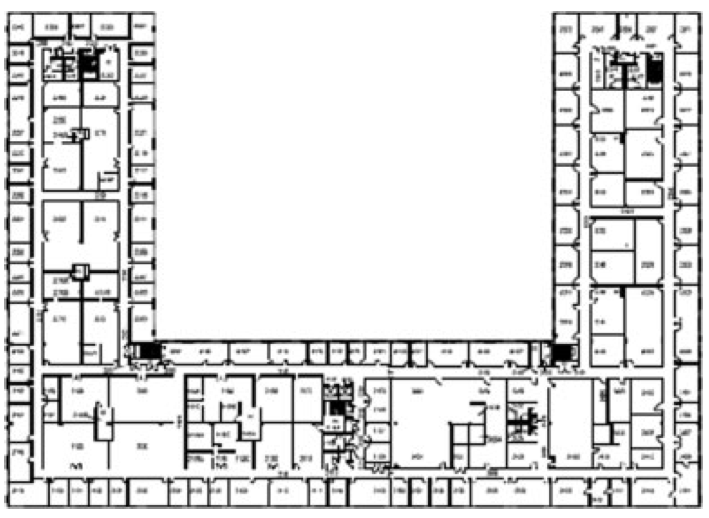
\includegraphics[width=0.5\textwidth]{images/grundriss.png}
    \caption{A. V. Williams Gebäude: Grundriss des zweiten Stocks~\cite{bepsi}.}
    \label{fig:grundriss}
\end{figure}
Da das Gebäude aus 4 identischen Etagen besteht, genügte es die Daten eines Geschosses zu erheben.
Dabei wurden unter anderem die Breiten und Längen von Korridoren, Türrahmen und Treppenhäusern
für die Approximation der Kapazitäten und Reisezeiten
ausgemessen sowie eine Netzwerkrepräsentation entwickelt. Fahrstühle wurden nicht berücksichtigt, da
der Gebrauch im Gefahrenfall untersagt ist. Zudem wurde auf eine Modellierung von Fensterausstiegen im
Erdgeschoss oder anderen Stockwerken verzichtet.
Nach der Überführung des Gebäudegrundrisses in ein Netzwerk, besteht dieses insgesamt aus 612 Knoten,
1480 Kanten und fünf Ausgängen. Um eine realistische Einschätzung für das Fassungsvermögen der
Räume (Vorlesungssäle, Büros, Labore) und den daraus resultierenden Flussraten zu erhalten,
wurde der NFPA 101 Life Safety Code \cite{fassungsvermoegen} herangezogen.
Die Flussrate wird für die später folgenden Testszenarien in drei Stufen unterteilt:
average (1), maximum (2) und maximum plus (3). Dabei wurden zur Schätzung der jeweiligen
Flussrate zum einen empirische Beobachtungen sowie Berechnungen \cite{pedestrian} und zum anderen charakteristische
Fußgängerbewegungen \cite{movement_params} mit einbezogen. Das Personenangebot orientiert sich am maximalen
Fassungsvermögen der Räume.\\
Anhand der Tabelle~\ref{tab:movement_params} wurden Näherungswerte für die Reisezeit sowie die
Kapazität der jeweiligen Kante ermittelt.
\begin{table}[htb!]
\centering
\caption{Bewegungsparameter für Gebäude \cite{movement_params}.}
\label{tab:movement_params}
\begin{tabular}[c]{|c|c|c|c|}\hline
 Verbindungsweg  & Dichte $[\frac{Personen}{ft^2}]$  & Geschwindigkeit $[\frac{ft}{min}]$ & Fluss $[\frac{Personen / min}{ft}]$   \\\hline\hline
  Tür   & 0.22 & 120 & 26  \\\hline
  Flur  & 0.20 & 120 & 24  \\\hline
  Treppe& 0.19 &  95 & 18  \\\hline
\end{tabular}
\end{table}
Die Tabelle macht deutlich, dass ein Treppenhaus weniger Menschen fassen kann als beispielsweise ein
Flur und dadurch die langsamste Alternative darstellt.

\section{Szenarien}
In diesem Abschnitt werden die sechs Testszenarien, die in Tabelle~\ref{tab:scenarios} aufgelistet sind und den
Testläufen zugrunde liegen, näher erläutert.
Die bei der Erstellung der Szenarien berücksichtigten Faktoren sind die initiale Personenanzahl an
den Quellknoten, Informationen darüber, ob Treppen und Flure passierbar sind oder nicht (arbeiten die Kanten
auf maximaler Kapazität bzw. Reisegeschwindigkeit) sowie die Art und der Ort des Ereignisses, welches die
Evakuierung ausgelöst hat.
Für alle Szenarien gilt $T = 20\,min$ (betrachteter Zeitraum) und dass alle Kanten initial frei sind.
\begin{table}[htb!]
\centering
\caption{Testszenarien}
\label{tab:scenarios}
\begin{tabular}[c]{|c|c|c|c|c|}\hline
  Szenario & Kapazitäten & Reisezeiten & Angebot & Gebäudezustand\\\hline\hline
  1 & 1    & 1    & 1 & ideale Bedingungen \\\hline
  2 & 1    & 1    & 3 & ideale Bedingungen \\\hline
  3 & 0.98 & 1.02 & 1 & leicht beschädigt \\\hline
  4 & 0.98 & 1.02 & 2 & leicht beschädigt \\\hline
  5 & 0.96 & 1.04 & 3 & beschädigt \\\hline
  6 & 0.95 & 1.06 & 3 & stark beschädigt, einige Wege unpassierbar \\\hline
\end{tabular}
\end{table}
Die ersten beiden Szenarien spielen unter idealen Bedingungen, allein das Personenangebot wird im zweiten
Fall angehoben. In der Realität würde dies beispielsweise eine Feuerübung simulieren.
Zudem wird der Gebäudezustand als gleichbleibend angenommen im Gegensatz zu den restlichen
Szenarien, die eine kontinuierliche Verschlechterung der Konditionen mit einbeziehen.
Dies geschieht, indem die aus der Tabelle~\ref{tab:scenarios} ersichtlichen Multiplikatoren für die Kapazität und
die Reisezeit in jedem Zeitschritt mit dem aktuellen Wert multipliziert werden.
Somit wird die Kapazität der Kanten stetig geringer und die Reisezeit größer.
Die Testfälle sind so entwickelt worden, dass sich der Gebäudezustand mit steigender Szenariennummer
verschlechtert und sich einem realistischen Szenario angenähert wird.
Dementsprechend sind die Bedingungen der Szenarien drei bis fünf ungünstiger als in den ersten beiden Fällen,
da sich diese über die Zeit verschlechtern, wobei noch keine realistische Gefahrensituation simuliert wird.
Erst im sechsten und letzten Fall werden realistische Szenarienwerte erreicht. Simuliert wurde ein
Feuerausbruch im Westflügel des vierten Stocks unter der Annahme, dass ein Korridor versperrt und die
nächste Treppe unpassierbar sei.\\
Die Ergebnisse des Benders Decomposition Algorithmus werden im folgenden Abschnitt dargestellt.

\section{Ergebnisse}
Der Benders Decomposition Algorithmus wurde in Microsoft Visual Studio C++ 6.0 implementiert und auf einem
PC mit einem Pentium $4$ CPU $3,20$ GHz und $2,0$ GB RAM getestet.\\
Die resultierenden Ergebnisse zeigt Tabelle~\ref{tab:ergebnisse}. In der ersten Spalte ist das jeweilige
Szenario aufgeführt, die zweite Spalte beschreibt die Anzahl der Iterationen bzw.\ die Anzahl der Benders
cuts und die Spalten drei und vier listen die Laufzeiten des Algorithmus in Sekunden auf, wobei
zum einen bei Erreichen von 95\,\%iger Optimalität abgebrochen wurde und zum anderen die optimale Lösung
berechnet wurde.
\begin{table}[htb!]
\centering
\caption{Ergebnisse für das reale Netzwerk}
\label{tab:ergebnisse}
\begin{tabular}[c]{|c|c|c|c|}\hline
  Szenario & Anzahl Cuts & bis 95\,\% Optimalität $[s]$ & bis Optimalität $[s]$  \\\hline\hline
  1 &  4 & -    &  3.0 \\\hline
  2 &  4 & 1.6  &  3.3 \\\hline
  3 & 12 & 1.9  & 30.8 \\\hline
  4 & 36 & 6.0  & 31.2 \\\hline
  5 & 32 & 19.6 & 58.5 \\\hline
  6 & 44 & 17.7 & 94.8 \\\hline
\end{tabular}
\end{table}
Aus der Tabelle ist ersichtlich, dass die Laufzeit mit schlechter werdendem Gebäudezustand
wie erwartet zunimmt.
Dabei ist interessant zu beobachten, dass die Rechenzeit bei steigendem Gebäudeverfall
weniger als linear ansteigt. Zudem benötigt der Benders Decomposition Algorithmus signifikant
weniger Zeit um eine 95\,\%ige Optimalität zu erreichen als bei der Berechnung der optimalen
Lösung. Im Fall einer Evakuierung müsste das \textit{BEPSI} zudem ständig neu gelöst werden,
da sich der Gebäudezustand vermutlich kontinuiertlich ändert (insbesondere das Personenangebot, die
Kantenkapazitäten sowie -reisezeiten).
Aus diesem Grund könnte es sinnvoll sein den Algorithmus bereits nach kurzer Zeit
abzubrechen (was kein Problem darstellt, da dieser immer eine gültige Lösung liefert),
um Zeit zu sparen und die zu evakuierenden Personen möglichst sofort mit den neusten Informationen zu versorgen.
Ist beispielsweise ein Treppenhaus eingestürzt, so will man dies den Personen auf dem Weg
dorthin nicht erst nach 95 Sekunden mitteilen und sie damit eventuell in eine Gefahrensituation
laufen lassen, sondern besser bereits nach 18 Sekunden.\\
Es sei zudem noch angemerkt, dass der BD Algorithmus mit einem hier nicht aufgeführten
\textit{Branch and Cut} Algorithmus verglichen wurde, wobei BD in jedem Fall deutlich
schneller war.


\chapter{Fazit}
\label{sec:fazit}
Abschließend folgt nun eine kurze Zusammenfassung in Verbindung eines kleinen Fazits.
Zunächst wurde das \textit{Building Evacuation Problem with Shared Information} beschrieben
und anschließend als gemischt-ganzzahliges lineares Programm formuliert.
Um dieses MIP zu lösen wurde das exakte Lösungsverfahren \textit{Benders Decomposition}
vorgestellt. Am Beispiel eines vierstöckigen, real existierenden Gebäudes wurde dieses
Verfahren demonstriert und seine Anwendbarkeit gezeigt.
Das \textit{BEPSI} bedient sich zwar bereits bekannter Verfahren, zeichnet sich aber
insbesondere durch die zuvor nie betrachtete Berücksichtigung der Gruppendynamik aus.
Personengruppen dürfen folglich nicht einfach an einem Knoten auf verschiedene Kanten
(Wege) aufgeteilt werden.
Zudem wird eine kontinuierliche Verschlechterung der Bedingungen in die Kalkulation
mit einbezogen (beispielsweise das dynamische Ausbreiten eines Feuers oder zerstörte
Gebäudestruktur). Dadurch können die zu evakuierenden Personen mit Hilfe ständiger
Liveupdates aus Gefahrensituationen oder um diese herum geleitet werden.\\
\\
Mögliche Ansätze der Verbesserung könnten zum Beispiel die Bestimmung der Kantenkosten
(Reisezeit) sein. Diese hängt aktuell nur vom Netzwerkzustand ab, nicht jedoch von der
Anzahl der Personen, die sich auf einer Kante befinden. Zudem muss der zu betrachtende
Zeitraum $T$ einer Evakuierung stets im Voraus angegeben werden. Dies kann unter Umständen
zu einem Problem führen, wenn dieser Zeitraum zu klein gewählt wird.\\
Da das vorgestellte Verfahren allgemein gehalten ist, kann es leicht auf andere
Einsatzgebiete übertragen werden. Denkbar ist beispielsweise die Evakuierung einer
geografischen Region aufgrund eines Militärangriffs, einer Naturkatastrophe oder
einer durch Menschen verursachten Katastrophe (Atomunfall).\\
Schließlich böte sich noch die Möglichkeit zur Entwicklung heuristischer Verfahren,
die deutlich schneller ein annähernd gutes Ergebnis für sehr große Netzwerke liefern, um somit
möglichst wenig Zeit dabei zu verlieren Menschen aus Gefahrensituationen zu führen.
Die optimale Lösung des \textit{BEPSI} könnte dazu als Richtwert (Benchmark) dienen, an dem
sich die Heuristiken messen.


\newpage
\singlespacing

\bibliography{literatur}
\bibliographystyle{alphadin}

\end{document}
